\chapter{Procedural Content Generation}
In the world of game development we strive to create the best experiences for a wide and diverse audience.
During the course of development there are a number of obstacles that can (and often will) hinder the progress of the developed game.
Some of these hindrances come from processes that are essential to a game like; level- and world building, or story- and quest design.
They take a proportionally large amount of development time and take a very specific mindset to create.

Content is a vague term, as it can be used do describe anything within a game.
Ranging from levels and quests, to textures and music, everything that the player can experience within a game is referred to as content.
Games such as the \gameby{Diablo}{Blizzard Entertainment} use content generation to rearrange dungeons with every play-through, and \gameby{Elder Scrolls IV: Oblivion}{Bethesda Game Studios} uses their \textit{Radiant Quest} to generate quests suited to the player.
The generation itself can take place at run-time starting a new generation during the actual game.
In this way the game can take a different form at any given time, making the game at least a little different for ever player on every play-through. 
Another possibility is to generate content during the development cycle.
This is mainly used to save development time, adding the benefit of creating an abundance of content that can be tweaked to create a more author-centric feel to the game.
The term \textit{Procedural} refers to the algorithms, and indeed procedures, used to generate the content.
These procedures should result in predictable content and range from using cellular automata for generating dungeons, as is the case with Rouge, or using a Voronoi/Delaunay dual-graph to generate realistic worlds.
A good example is is the card game \game{Klondike}, alternatively called \game{Solitare}/\game{Patience}.
In this simple card game, shuffling the deck is the procedure used to randomly reorder the cards with the resulting 'content' being the layout of the game.

Procedural content generation can be a viable option to spice up a game or help cut development time for various tasks.
But it should be noted that the use of PCG is dependant upon the game that's being produced.

Rouge, as a \rogue, depends heavily on procedural content generation to serve new maps and levels to explore. \textit{Roguelikes} are designed to be played over and over again, teaching the player to master the mechanics of the game, but not to memorize the worlds in which they play. In the spirit of research we ask the question: "Why does Rouge need procedurally generated content?"

\section{Rouge}
\label{sec:PCG:Rouge}
\begin{quotation}
\textsl{You are a nameless traveller that has been compelled to search for something.
An object, a person, or just a place.
You don't know yet, but it's up to you to find out.
You will travel through various caves, forests and towns to pursue the whims of your heart.
Every time you seem to solve a problem, another one turns up.
Always moving you towards some inevitable doom.
Are you born for heroism, or will you die unloved and unknown?
\\\\
Choose your path, and see where the voices in your head take you.}
\end{quotation}
Rouge is a tile-based \rogue game where the player travels through the world to discover a myriad of people and monsters that will react to the player in different ways depending on the players attributes. 
The setting is that the main character is a neurotic, or maybe even a little insane, adventurer.
Voices in his head give him instructions (by way of the narrative planner) to do things.
This can be finding an item, talking to a person, or beating up some monsters. 
In Rouge you play out the life of this character, and after he dies another person with the same affliction will become available for play. 

\subsection{Mechanics}
Rouge is played in turns, with each action ending that character's turn. 
The main exception is movement; a character can move as many tiles as their speed attribute allows. 
An example would be that the player always starts with a speed of two, and thus can walk two tiles during \his respective turn. 
Monsters in the starting area will have a speed of one, ensuring that the player will always move faster. 
Speaking to NPCs, fighting monsters and picking up items all cost a turn. 

The items a player picks up can either be equipped or used, with a variety of bonuses and penalties. 
As seen in figure~\ref{fig:quest} the player is wearing some armour and is holding a combat-knife and shield. 
Attacking monsters would increase the player's attributes in the respective categories of the equipped items. 
In this instance, the armour and helm grant the player bonuses on defence, but penalties on speed, every time \he equips heavy armour. 
The combat-knife will grant extra strength on small weapons, and so forth. 
Finding the right items contribute to making a character that suits the player's play style. 

Getting a high score on a particular attribute will make NPCs behave differently around you. 
An example would be a hunter that is severely impressed with your archery skill, and give you his prized bow to use. 
But figure~\ref{fig:convo} shows us an NPC that is annoyed at the player for bringing an equipped weapon in to his house, and he would refuse giving the player information or items while in this state.


\begin{figure}[p]
	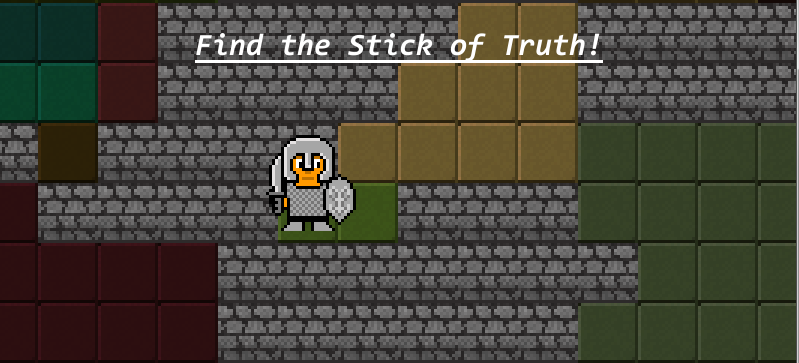
\includegraphics[width=\textwidth]{gameplay/Quest}
	\caption{The narrator telling the player what to do.}\label{fig:quest}
\end{figure}
\begin{figure}[p]
	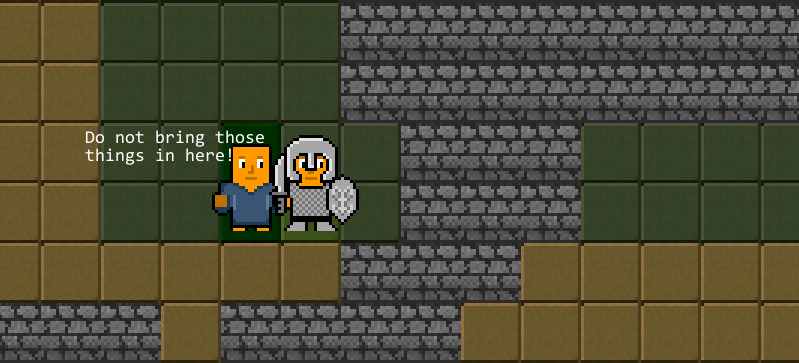
\includegraphics[width=\textwidth]{gameplay/convo}
	\caption{A NPC that is angry at the player for carrying a weapon in his home}\label{fig:convo}
\end{figure}
\begin{figure}[p]
	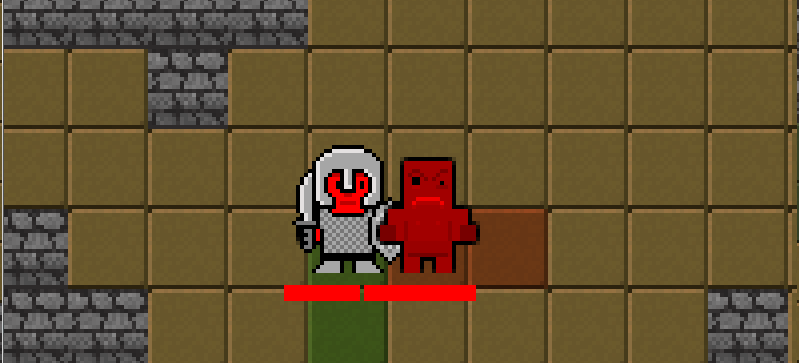
\includegraphics[width=\textwidth]{gameplay/attack}
	\caption{The player and a monster attacking each other}\label{fig:attack}
\end{figure}

\section{World generation}
\label{sec:world_gen}
Rouge can be played two ways; either with a persistent world or a generative one. 
In this chapter we will focus on the generative worlds and the persistent world will be covered in chapter~\ref{ch:planning}.

Creating worlds in Rouge could be done a multitude of ways; either manually, dynamically generated, or generated for static purposes. 
Static generation means that the designer generates content that \he can tweak and polish, fine-tuning it for purpose.
Dynamic generation gives little control, every time a new game starts new content is generated. Dynamic generation limits the fine-tuning options that static generation has, but creates more novel content without the developers intervention.

The world within Rouge is dynamically generated to facilitate a large number of new worlds. If the developer had to manually create all the levels used within Rouge, either \he would just have one level, or \he would have to spend more time developing levels than developing the game itself. The second pressing reason for choosing a generative approach in contrast to a manual one is that level design might not be the designer's strong point, whereas software development is. 

\section{Cellular Automation}
When level design isn't favourable, automating that process is.
There are multiple well-known algorithms that solve this particular problem including but not limited to; \textit{the drunken walk}, maze algorithms, and cellular automata.
For the the world generation within Rouge I used a cellular automaton, for it's tried and tested use within other roguelike games and because I found it more technically challenging.
Celullar automata work by defining a regular grid of cells, each in any number of states. Using rules pertaining to the neighbours of each cell, that cell can change its state. For example; we define the states \textit{alive} and \textit{dead}. After that we define several rules:
\begin{enumerate}
	\item A cell goes into a \textit{dead} state when it has \underline{less} than 2 live neighbours.
	\item A cell goes into a \textit{dead} state when it has \underline{more} than 3 live neighbours.
	\item A cell goes into a \textit{alive} state when it has \underline{exactly} 3 neighbours.
\end{enumerate}
With these definitions set the grid could be populated with a random amount of cells in live state, assuming that the dead state is the default. Each step of the automaton will cycle through the rules, checking to see if the conditions of a rule is set. After all the cells have been checked the rules execute and changes the grid. With these three simple rules, we can generate moving shapes and repeating patterns. The rules come from one of the most recognized cellular automata; \game{Conway's Game of Life}. Figure~\ref{fig:game_of_life} shows an example of the emergent behaviour that these simple rules generate.


\begin{algorithm}[p]
	\KwIn{tilemap}
	\KwOut{new tilemap}
	let \textit{deadCells} and \textit{liveCells} be an empty collection of tiles\;
	\ForEach{tile in tilemap}{
		\uIf{tile.neighbours $\geq$ 5}{
			liveCells.push(tile)\;
		}\uElseIf{tile.neighbours $\leq$ 1}{
			deadCells.push(tile)\;
		}
	}
	\ForEach{tile in deadCells}{
		tile.alive = false\;
	}
	\ForEach{tile in liveCells}{
		tile.alive = true\;
	}
	\caption{Cellular Automation algorithm as used in Rouge}\label{alg:ca}
\end{algorithm}


During a step of this automaton, the algorithm walks through the game world and checks each tile for certain conditions pertaining to their neighbours. If these conditions are met, his state will be changed accordingly. The states a tile has in Rouge are a simple \textit{Wall} or \textit{Normal} state. When a tile has 5 or more wall neighbours, that tile itself becomes a wall. However, when a tile has less than 2 wall neighbours, the tile becomes a normal. The first rule ensures that tiles group together, and the other rule destroys any singular 'island' walls.

As we will discuss in chapter~\ref{ch:dml} a game made with the \diage system contains several entities.
One of those entities is a \textit{Space}.
Spaces represent any or all spaces currently within a game-world, ranging from a single room to a entire city or even the world. Spaces in Rouge are designated areas where the player can find shops and resolve \his objectives. These 'rooms' are generated using a simple tile-based flood-fill algorithm that circles around a selected tile. The algorithm has a maximum allowance that gets depleted by a tile's cost. This cost is higher for tiles that have fewer live neighbours than those that are encircled by them. This creates the effect that corridors are more expensive to fill (thus have a lower grouping rate) and large open spaces are easy to fill all the way through.

\begin{figure}[p]
	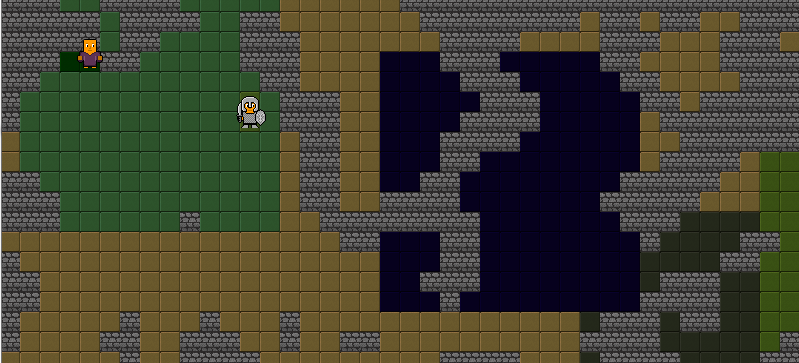
\includegraphics[width=\textwidth]{gameplay/spaces}
	\caption{Space entities depicted by the areas with coloured tiles}\label{img:gameplay:spaces}
\end{figure}


\section{Evaluation}
We started discussing Rouge by asking the question: "\textit{Why does Rouge need procedural content techniques}". 
Section~\ref{sec:PCG:Rouge} stated that world building could be done in three different ways; manual, dynamic generation, and static generation where I chose the dynamic route.
This choice was made by the requirements that the game had.
The game needed new worlds/levels for every new game that started. 
The manual option meant the designer had to develop all the worlds by hand, taking in a lot of time. 
Static generation would have given me a set of maps that the designer could polish into perfectly crafted worlds, which would be faster than manual creation and giving me pretty much the same results.
Dynamically generating the worlds meant there would be more time implementing a more crucial element of the game: The narrative planner. 

%The world itself isn't a key point in the development of Rouge, and is therefore fine by being 'suboptimal'.

\begin{figure}[p]
	\centering
	\begin{subfigure}[b]{0.3\textwidth}
		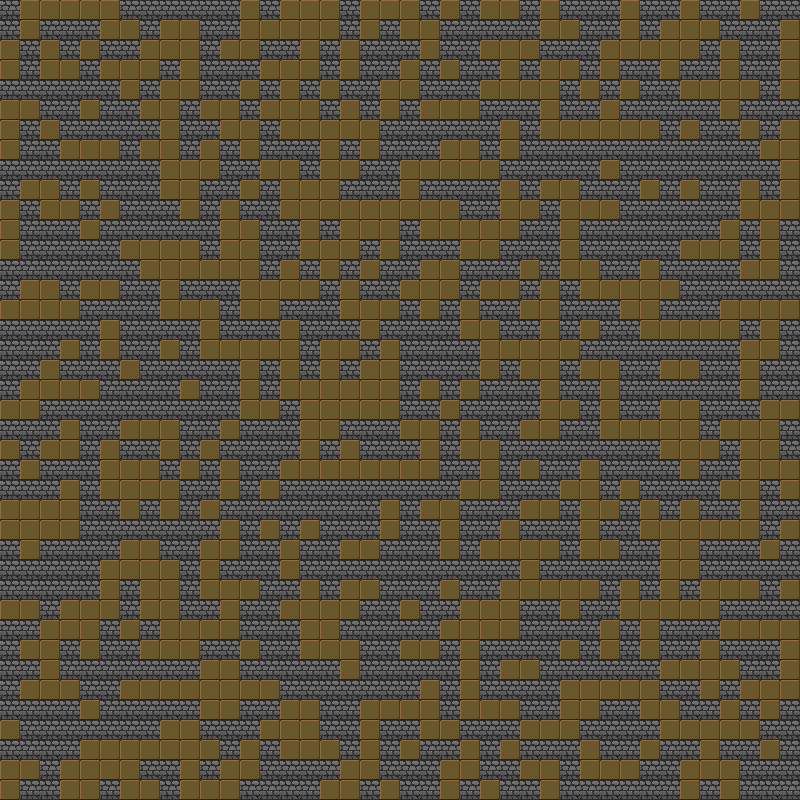
\includegraphics[width=\textwidth]{rouge/screenshot0}
		\caption{Initial map}
	\end{subfigure}	
	~
	\begin{subfigure}[b]{0.3\textwidth}
		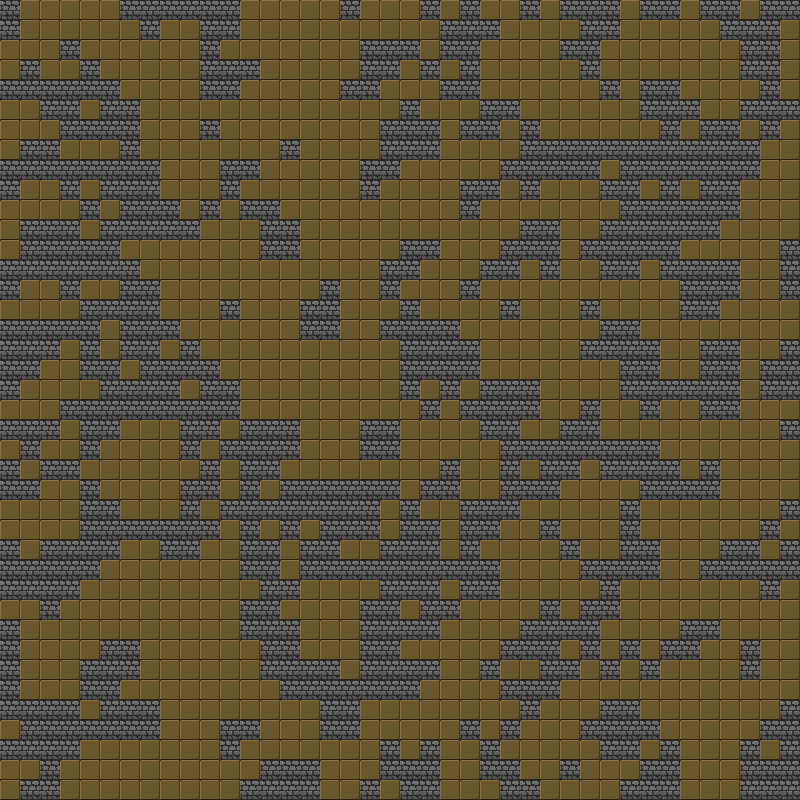
\includegraphics[width=\textwidth]{rouge/screenshot1}
		\caption{Step 1}
	\end{subfigure}	
	~
	\begin{subfigure}[b]{0.3\textwidth}
		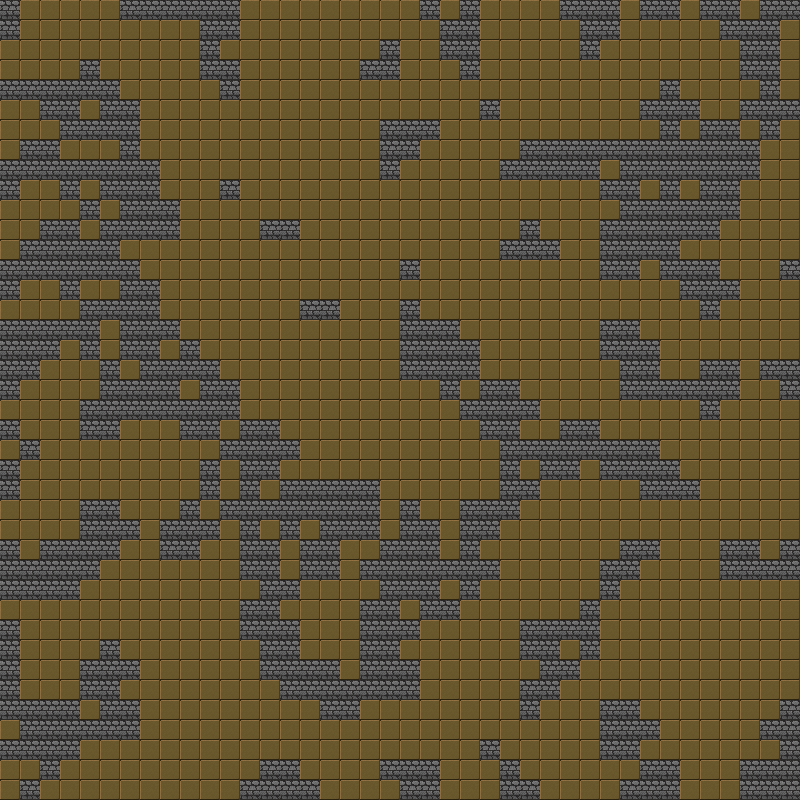
\includegraphics[width=\textwidth]{rouge/screenshot2}
		\caption{Step 2}
	\end{subfigure}	
	~
	\begin{subfigure}[b]{0.3\textwidth}
		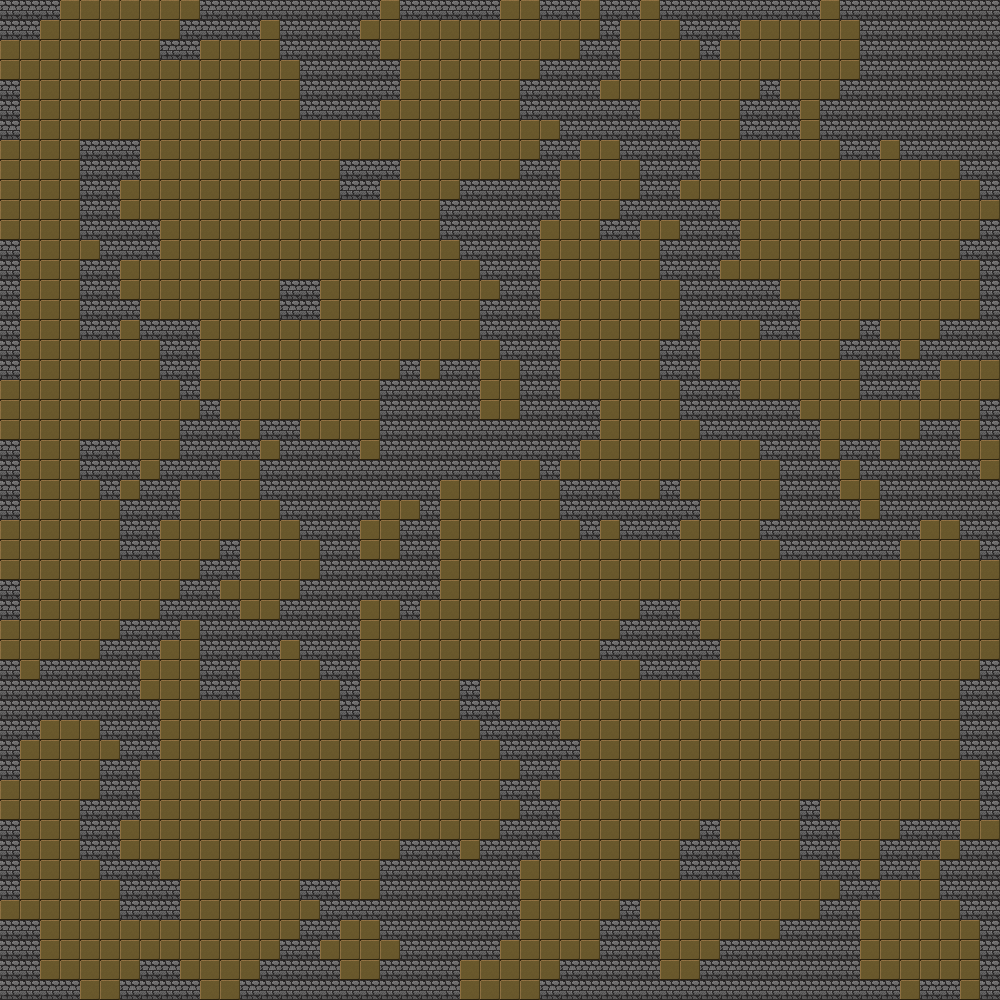
\includegraphics[width=\textwidth]{rouge/screenshot3}
		\caption{Step 3}
	\end{subfigure}		
	~
	\begin{subfigure}[b]{0.3\textwidth}
		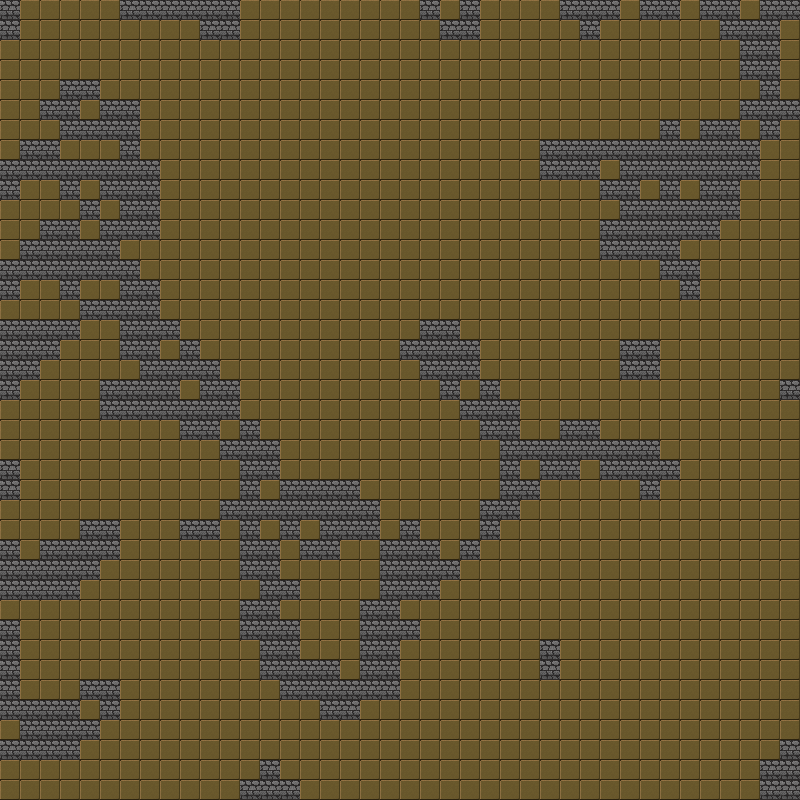
\includegraphics[width=\textwidth]{rouge/screenshot4}
		\caption{Step 4}
	\end{subfigure}
	~
	\begin{subfigure}[b]{0.3\textwidth}
		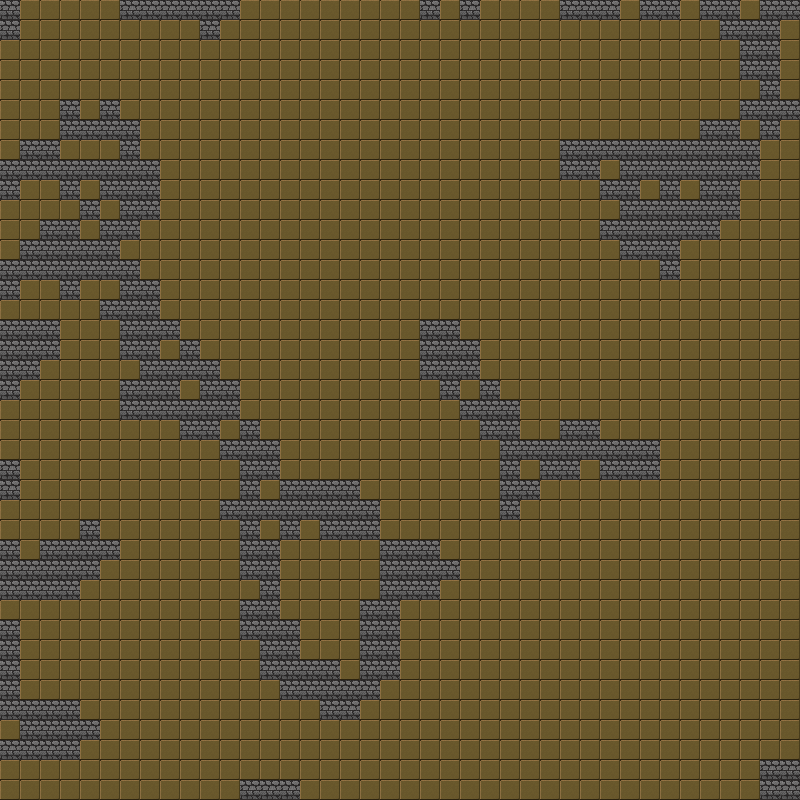
\includegraphics[width=\textwidth]{rouge/screenshot5}
		\caption{Step 5}
	\end{subfigure}	
	\caption{The generation of a world in Rouge}\label{fig:rouge:screens}
\end{figure}

\begin{figure}[p]
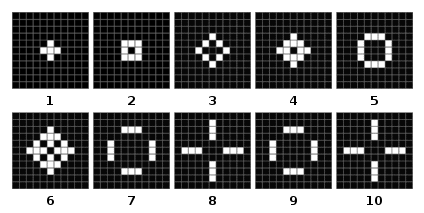
\includegraphics[width=.8\textwidth]{gameoflife}
\caption{An example of the Game of Life generation steps}\label{fig:game_of_life}
\end{figure}


%\section{Narrative}
%I want to go as far as to say that narration defines what being humans means.
%We, as a society and as a species, have always used a storytelling context to receive and deliver information.
%Be that a story on the dangers of bears and lions to a more modern setting for the sake of leisure.
%But even then, for the sake of argument we need a proper definition of a narrative.
%Riedl and Young stated that a narrative is in it's simplest form a temporally ordered sequence of events \citep{Riedl:2004:IPM:1018409.1018753}.
%This is the definition I will keep to throughout this document.
%One other thing of particular note; a narrative does not explicitly mean the usage of text or spoken word.
%This is an easy, and clear way to convey a story, but never the only ways to do so.
%Granted; it can certainly add to the experience, but in my own opinion a game should, first and foremost, try to convey a story through it's mechanics.
%To discard that rule is to introduce the expensively named \textit{ludo-narrative dissonance}, or a discord between narrative and game-play.
%Games can be a powerful medium in which to explore the human condition, but for that we can really come to that point we need to start treating it with that same respect.
%\section{Static and dynamic generation}
%\label{sec:static_dynamic_generation}
%Throughout this document I reference to static and dynamic generation, or static and dynamic narratives.
%These terms refer to the point in time where the generation takes place.
%When we speak of a static generation, this happens during the development.
%A developer may choose to generate a game world and continue to populate that world with the rest of his content.
%In a dynamic setting, said world is generated at runtime, usually when a new game is started.
%This means that every time the player starts a new game he gets a new world to explore.
%In a narrative context that means that a static narrative has been generated, but will never change.
%Whereas a dynamic narrative will always try to be different from the former.